Fundamentale Fragen:
\begin{itemize}
	\item Was ist Entscheiden?
	\item Welche Arten von Systemen fällen Entscheidungen?
	\item Welche ist der allgemeinste Rahmen für eine Definition von Entscheidungssystemen?
\end{itemize}

\subsection{Der rationale Agent}
\begin{itemize}
	\item Allgemeine Definition eines in eine Umwelt eingebetteten, handelnden Systems
	\item Beliebige Art von Umwelt
	\item Definiert durch den Agentenzyklus: \textbf{Perzeption -- Entscheidung -- Handlung} (\autoref{ch07_agentenzyklus})
	\item Der Agentenzyklus ist eine andere Darstellung eines Regelkreises
	\item Entscheidung ist eine abstrakte Form der Regelung
\end{itemize}

\begin{figure}[ht]\centering 
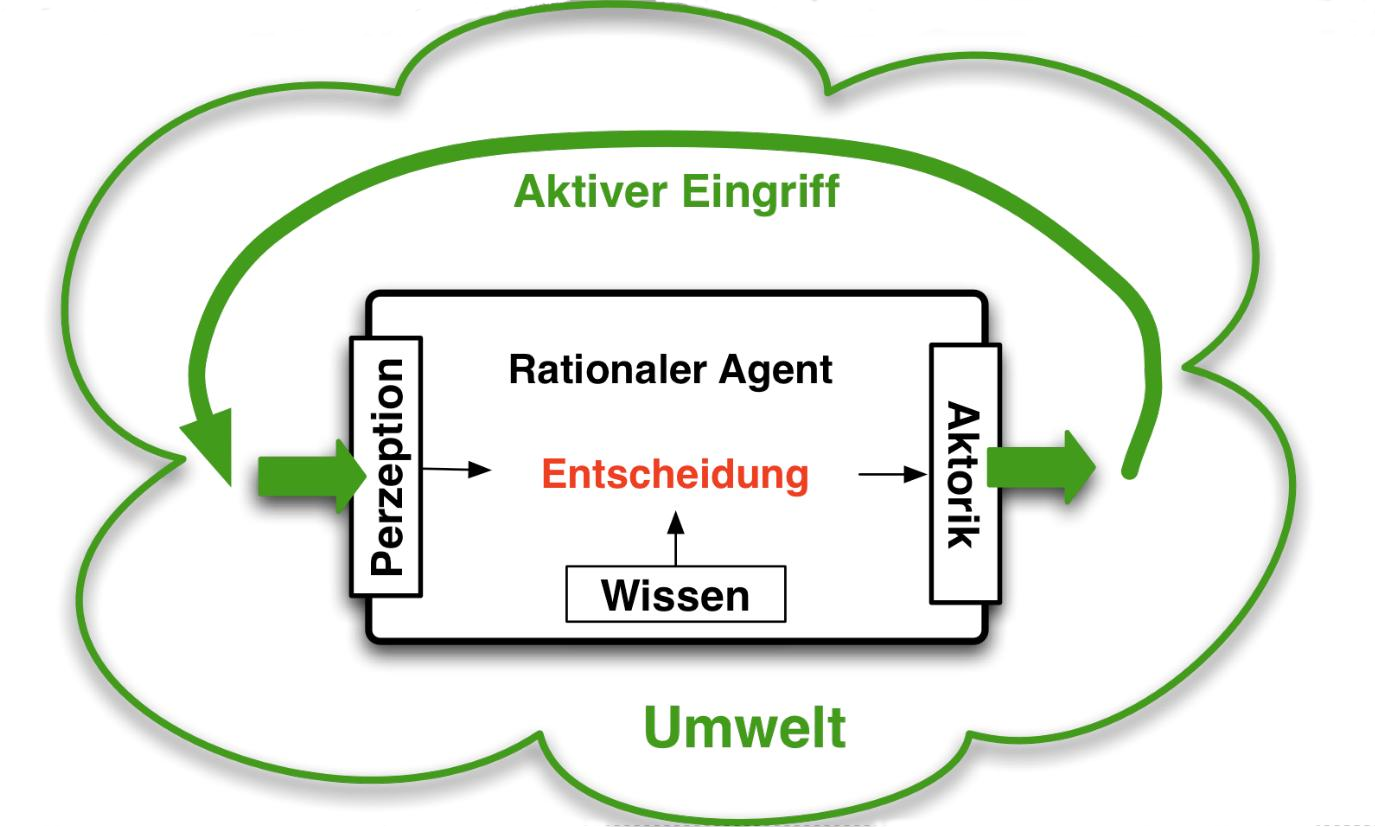
\includegraphics[width=0.8\textwidth]{figures/07_agentenzyklus.png}
\caption{Der Agentenzyklus: Jede Modellbildung der Welt ist starke Reduktion}
\label{ch07_agentenzyklus}
\end{figure}

\subsubsection{Beispiele}
\paragraph{Schachcomputer}
\begin{itemize}
	\item Keine physische Umwelt
	\item Sehr beschränkte Umwelt
	\item Nur ein Ziel: das Spiel zu gewinnen
	\item Sensorik: Das Spielfeld wird komplette wahrgenommen
	\item Aktorik: Durchführung eines symbolischen Zugs
	\item Umwelt: semi-statisch, episodisch, diskret, deterministisch, vollständig beobachtbar, Multiagent
\end{itemize}
\paragraph{Industrieroboter}
\begin{itemize}
	\item Oftmals, bei Abwesenheit von Sensorik, kein Agent, sondre nur ein Werkzeug
	\item Physische Umwelt
	\item Beschränkte Umwelt
	\item Wenn überhaupt rationaler Agent, üblicherweise extrem begrenzter Entscheidungsrahmen
	\item Ziel: Erfolgreiche Ausführung einer Operation
	\item Umwelt: dynamisch, episodisch, diskret oder kontinuierlich, deterministisch, vollständig beobachtbar, Einzelagent oder Multiagent
\end{itemize}
\paragraph{Mensch}
\begin{itemize}
	\item Extrem komplexe Umwelt
	\item Sehr mächtige Perzeption
	\item Sehr wissensbasiert
	\item Vielschichtige Motivationen und Zielsetzungen
	\item Umwelt: dynamisch, sequentiell, kontinuierlich, stochastisch, unvollständig beobachtbar, Multiagent
\end{itemize}
\paragraph{Serviceroboter}
\begin{itemize}
	\item Anforderungen dem Menschen viel ähnlicher als einem Industrieroboter
	\item Sehr komplexe Umwelt
	\item Vielschichtige Zielsetzung
	\item Es ist bei Servicerobotern ein ganz anderes Vorgehen, als bei Industrierobotern erforderlich
	\item Umwelt: wie beim Menschen
\end{itemize}

\subsubsection{Umwelt}
Für die verschiedenen Agenten werden sehr unterschiedliche Umgebungen benötigt.
Ein Rahmen für eine nützliche und eindeutige Charakterisierung von Umgebungen ist nötig.
\paragraph{Anforderungen}
\begin{itemize}
	\item Die Charakterisierung muss fundamentale, nicht oberflächliche Eigenschaften aufzeigen
	\item Es muss ein Rahmen gebildet werden, in den verschiedenen Verfahren und Paradigmen eingeordnet werden können
	\item eine Leitlinie für die Entwicklung neuer Verfahren muss gebildet werden
\end{itemize}
Umwelten verschiedener Agenten können gut durch einige fundamentale, duale Eigenschaften unterschieden werden.
\paragraph{Eigenschaften} \mbox{}
\vspace{1em} \\
\begin{tabular}{p{0.4\textwidth} p{0.1\textwidth} p{0.4\textwidth}}
\textbf{statisch} & \centering vs.\ & \textbf{dynamisch}\\
Der Agent ist das einzige Element, welches den Zustand der Umwelt verändert
& &
Die Umwelt kann sich auch ohne zutun des Agenten verändern
\\
\textbf{episodisch} & \centering vs.\ & \textbf{sequentiell}\\
Der zeitliche Verlauf des Geschehens  ist in abgeschlossene Einheiten unterteilt, zwischen denen keinerlei kausal Zusammenhänge bestehen
& &
Die vollständige zeitliche Vergangenheit hat Auswirkungen auf die Gegenwart ,die Gegenwart auf die gesamte Zukunft
\\
\textbf{diskret} & \centering vs.\ & \textbf{kontinuierlich}\\
Die Zustände der Umwelt sind diskret, ebenso der zeitliche Verlauf des Geschehens
& &
Der Zustandsraum der Umwelt ist kontinuierlich und die Zeit fließt ebenfalls kontinuierlich
\\
\textbf{deterministisch} & \centering vs.\ & \textbf{stochastisch}\\
Der Ausgang einer jeden Handlung ist eindeutig bestimmt
& &
Eine Handlung kann mit bestimmten Wahrscheinlichkeiten zu verschiedenen Ausgängen führen
\\
\textbf{vollständig beobachtbar} & \centering vs.\ & \textbf{unvollständig beobachtbar}\\
Der Agent kann die komplette Umwelt jederzeit vollständig und exakt wahrnehmen
& &
Der Agent kann die Umwelt nur eingeschränkt und fehlerbehaftet wahrnehmen
\\
\textbf{Einzelagent} & \centering vs.\ & \textbf{Multiagent}\\
Nur eine als Agent modellierbare Entität agiert in der Umwelt
& &
Viele als Agenten modellierbare Entitäten agieren in der Umwelt und können kooperieren oder konkurrieren
\end{tabular}
\\ \\
Die Beschreibung der Umwelt durch das jeweils komplexere Merkmal wird nur gewählt, wenn das einfachere Merkmal im Szenario des Agenten keine hinreichende Beschreibung ist.\\
\textit{Hinreichend} ist hierbei auch in dem Sinne zu verstehen, dass es oftmals noch keine ausreichenden Verfahren gibt, um die komplexeren Merkmale zu berücksichtigen.

\subsubsection{Utility -- Motivation des Agenten}
\begin{itemize}
	\item Ein Agent benötigt Motivation um Absichten als Fundament für Entscheidungen
	\item In der Entscheidungstheorie durch das Konzept der \textbf{Utility} abgebildet (Ursprung des Begriffs in der Ökonomie)
	\item Dieses Konzept ist deutlich allgemeiner, als spezielle Ziele z.B.\ in der logikbasierten Planung	
\end{itemize}

\paragraph{Konzept der Utility}
\begin{itemize}
	\item Die utility (auch: \textit{utility function}) modelliert in der Ökonomie ein numerisches Maß der Befriedigung eines Agenten (Menschen) durch einen bestimmten Konsum
	\item In der Robotik/KI wird jedoch ein Motivationsmaß eines Agenten nicht \emph{modelliert}, sondern \emph{konstruiert}
	\item Die uitility wird hier genutzt, um einem künstlichen Agenten bestimmte Motivationen einzupflanzen
	\item Die utility ist ein allgemeines Konzept: es können konkurrierende und ergänzende Zielsetzungen fusioniert werden
	\item Im Rahmen der utility können auch Absichten gegeneinander abgewogen werden
\end{itemize}

\subsubsection{Problem}
Die urspr\"ungliche, klassische Aktionsplanung nimmt an, dass die Umwelt statisch, episodisch, diskret, deterministisch und vollst\"andig beobachtbar ist und zudem konkreten, nicht \"uberlappenden Ziele verfolgt. 
F\"ur eine dynamische, sequentielle und kontinuierliche Umwelt gibt es Erweiterungen des klassischen Aktionsplanens, im Hinblick \textbf{stochastisch}, \textbf{vollst\"andig beobachtbar} und \textbf{unterschiedlich stark konkurrierende Ziele} jedoch nicht.
%
\begin{figure}[ht]
	\centering 
	\begin{subfigure}{.45\textwidth}
		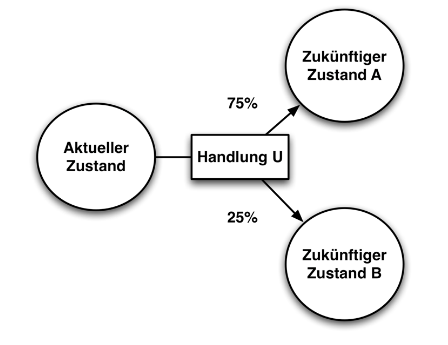
\includegraphics[width=\textwidth]{figures/ch07_stochastischeUmwelt.png}
		\caption{Stochastische Umwelt}
		\label{ch07_stumwelt}
	\end{subfigure}
	\begin{subfigure}{.4\textwidth}
		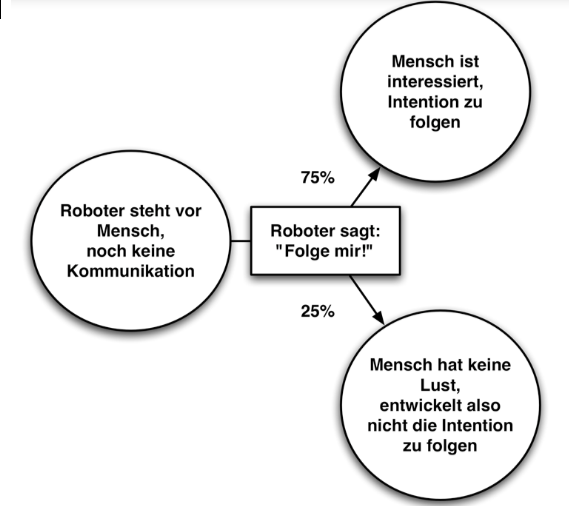
\includegraphics[width=\textwidth]{figures/ch07_umwelt-bsp.png}
		\caption{Beispiel}
		\label{ch07_umwelt-bsp}
	\end{subfigure}
	\caption{}
\end{figure}

\autoref{ch07_stumwelt} zeigt eine stochastische Umwelt.
\"Ubergangswahscheinlichtkeiten beschreiben hierbei den Ausgang von Handlungen.
In stochastischen Umgebungen ist daher es essenziell, dass mit numerischen Wahrscheinlichkeiten umgegangen werden kann, jedoch ist das in der klassischen, logikbasierten Aktionsplanung nicht der Fall, weshalb \textbf{probabilistische Methoden} (wie MDPs) zum Einsatz kommen.
%Exkurs zu Bayes F29+30
\subsection{Markov Prozesse}
\begin{itemize}
\item ein verbreitetes Werkzeug f\"ur die Modellierung stochastischer Prozesse
\item zentrale Eigenschaft: die zuk\"unftige Entwicklung kann durch Kenntnis einer \textbf{begrenzten} Vorgeschichte prognostiziert werden
\item erst diese Markoveigenschaft erlaubt die Prognose bez\"uglich der Zukunft in einem solchen stochastischen Prozess
\item es gibt zwei Arten von Markov Prozessen: zeitdiskrete und zeitstetige Markov Prozesse
\end{itemize}

\paragraph{Zeitdiskreter Markov Prozess:}
\begin{itemize}
\item werden auch Ketten genannt
\item \"Uberg\"ange in einer Markov Kette sind Spr\"unge in einer diskreten Zeit
\item Mathematisch wird die Wahrscheinlichkeit f\"ur einen zuk\"unftigen Zustand als bedingte Wahrscheinlichkeit, abh\"angig von einer endlichen Zahl an vergangenen Zust\"anden modelliert
\item die Ordnung einer Markov Kette gibt an, welcher Ausschnitt der Vergangenheit eine Rolle spielt
\item die Ordnung ist immer endlich, sonst w\"are die Markov Eigenschaft nicht erf\"ullt
\item je geringer die Ordnung, desto einfach die Modellierung
\end{itemize}
\newpage
\textbf{Markovkette 1. Ordnung} (Beispiel in \autoref{fig:ch07:mk-bsp})
\begin{itemize}
\item nur die Gegenwart spielt eine Rolle f\"ur die Betrachtung der Zukunft
\item die Wahrscheinlichkeit des Nachfolgezustands h\"angt nur vom aktuellen Zustand ab
\item $Pr(X_{n+1} = x | X_n = x_n, \ldots, X_1 = x_1, X_0 = x_0) = Pr(X_{n+1}|X_n = x_n)$
\end{itemize}
\begin{figure}
	\centering
  	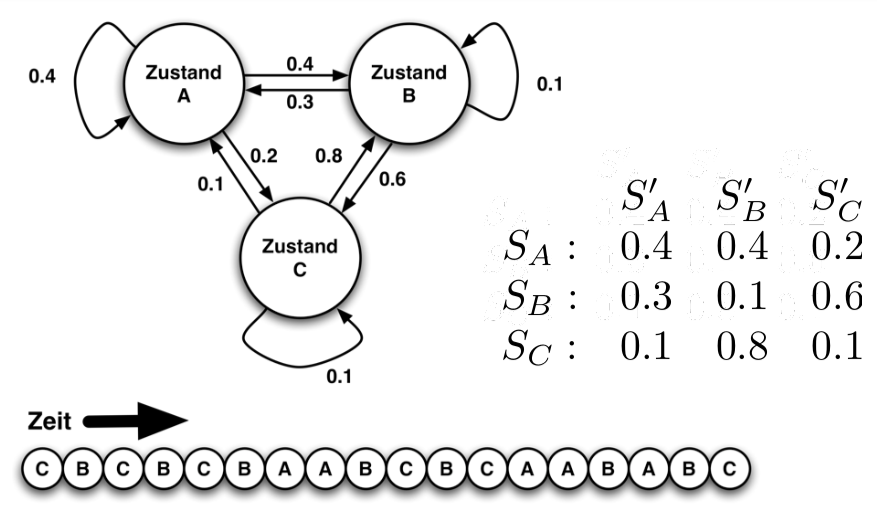
\includegraphics[width=0.5\linewidth]{figures/ch07_mk-bsp.png}
	\caption{Beispiel -- Markovkette 1. Ordnung}
	\label{fig:ch07:mk-bsp}
\end{figure}
Markovketten: Modellierung der Welt
\begin{itemize}
	\item Markovketten k\"onnen von Agenten zur Modellierung von stochastischen Umgebungen genutzt werden
	\item Bei diskreten Markovketten muss die Welt dazu in eine diskrete Zustandsmenge zerlegt werden
	\item Die Zerlegung kann f\"ur verschiedene Umweltaspekte getrennt erfolgen, z.B. Roboterposition, Objektform oder Intention eines Menschen
	\item Welt als diskrete Zust\"ande: einfache Beispiel: Unterteilung von R\"aumen in diskrete Regionen (die Position eines mobilen Roboters wird durch die Region, in der er sich befindet, repr\"asentiert)
	\item Welt als stochastischer Prozess: Bestimmte \underline{Ausl\"oser} f\"uhren zu stochastischen Zustands\"uberg\"angen (Bayesianische Modellierung), z.B. Handlung eines Agenten:\\ Beispiel:
	\begin{itemize}
		\item Der Roboter steht vor einem Mensch, es fand noch keine Kommunikation statt
		\item M\"oglichkeit 1: Roboter sagt: Folge mir!; damit ergibt sich eine Wahrscheinlichkeit von $75\%$, dass der Mensch interessiert ist und die Intention hat zu folgen und $25\%$, dass der Mensch keine Lust hat, also nicht die Intention entwickelt zu folgen
		\item M\"oglichkeit 2: Roboter sagt: Ich habe etwas interessantes zu zeigen. Folge mir bitte!; damit steigt die Wahrscheinlichkeit, dass der Mensch folgen will auf $90\%$, wohingegen er mit $10\%$iger Wahrscheinlichkeit nicht folgen will
		\item d.h. durch die Wahl der Handlung kann der Agent die \textbf{\"Ubergangswahrscheinlichkeiten steuern}!!! (Siehe auch \autoref{fig:ch07:weltmode-bsp}).
	\end{itemize}
\end{itemize}
\begin{figure}[!h]
	\centering
  	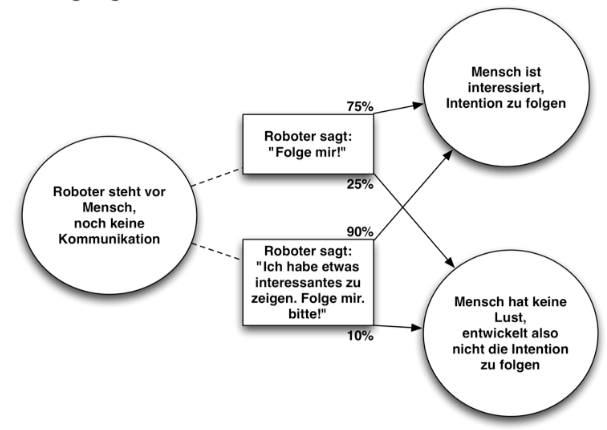
\includegraphics[width=0.5\linewidth]{figures/ch07_weltmode-bsp.png}
	\caption{Verschiedene Auslöser haben unterschiedliche Übergangswahrscheinlichkeiten. Durch die Wahl der Handlung kann der Agent die Übergangswahrscheinlichkeiten steuern.}
	\label{fig:ch07:weltmode-bsp}
\end{figure}
\subsubsection{Markov Entscheidungsprozesse}
Ketten von Handlungen bzw. Ausl\"osern f\"uhren zu Bayes-Netzwerken. F\"ur die Entscheidungsfinder in diesen stochastischen Prozessen existiert ein fundiertes Modellierungsrahmenwerk spezieller Bayes-Netze: \textbf{Markov Decision Processes} (MDPs). Hierbei kann der Agent, im Unterschied zu Markov-Ketten, aktiv Entscheidungen treffen.

\paragraph{Struktur}
\begin{itemize}
\item Eine Menge von symbolischen \textbf{Zust\"anden} der Welt $S$ (d.h. die Umwelt bei einem MDP ist diskret)
\item Eine Menge von symbolischen Handlungen des Agenten $U$
\item Ein \textbf{\"Ubergangsmodell} (transition model) $T(s', u, s)$ welches die stochastischen \"Uberg\"ange modelliert, also das Verhalten der Welt aufspannt (modelliert den Markov-Prozess). Hierbei ist die Frage, wie wahrscheinlich ein bestimmtes Ergebnis folgt, wenn in einem beliebigen Zustand eine beliebige Handlung ausgeführt wird. Das Modell muss vollständig definiert werden (d.h.     Unmöglichkeiten haben die Wahrscheinlichkeit 0).
\item Ein \textbf{Belohnungsmodell} (reward model) $R(s,u)$ welches die Ziele und Absichten des Agenten modelliert. Auch negative Belohnungen/Strafen möglich. 
\item Ein \textbf{Startzustand} $s_0$
\end{itemize}
Zust\"ande und Aktionen m\"ussen dabei einzigartig sein.
Es gilt au{\ss}erdem die Markov-Eigenschaft, d.h. alle Wahrscheinlichkeiten h\"angen immer nur vom aktuellen Zustand ab und nicht von den bereits vergangenen.
Die in jedem Schritt aufaddierte Belohnungen werden \emph{Utilitiy} genannt und die Aufgabe des Agenten besteht darin, Aktionen mit hoher Belohnung zu w\"ahlen, um die Utility zu maximieren.

\paragraph{Statische Eigenschaften}
\begin{itemize}
	\item In einem MDP ist die Welt zu jedem Zeitpunkt in \textbf{genau einem} Zustand (und nur in diesem, kein fuzzy Zustand, keine Wahrscheinlichkeits-Verteilung über mehrere Zustände
	\ita brauche in echter Umgebung Diskretisierungsverfahren für kontinuierlichen Zustandsraum, im Zweifelsfall führe einen Restzustand \glqq other\grqq{} ein
	\item In einem diskreten MDP ist dies ein symbolischer Zustand, welcher alle Eigenschaften der Welt repr\"asentiert
	\item Der Agent kann in jedem Agentezyklus \textbf{genau eine} Handlung ausf\"uhren
	\item In einem diskreten MDP (diskrete Zeit) ist dies eine symbolische Handlung (kann auf tieferer Ebene aus mehreren Subhandlungen bestehen)
	\item Im reinen MDP nimmt der Agent den aktuellen Zustand \textbf{immer und eindeutig} wahr
\end{itemize}
\begin{figure}[!h]
	\centering
  	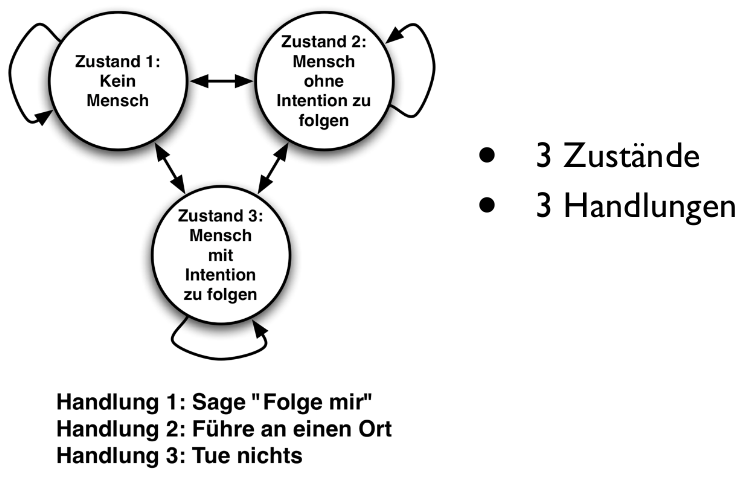
\includegraphics[width=0.5\linewidth]{figures/ch07_stat-bsp.png}
	\caption{MDP Beispiel -- statische Eigenschaften; hier für einen Museumsroboter welcher z.B. Möglichkeiten für Tracking und Dialogerkennung zur Aufbereitung des abstrakten Zustands hat (wenn der Mensch etwas gesagt hat hat er eher die Intention zu folgen)}
	\label{fig:ch07:stat-bsp}
\end{figure}
\paragraph{Transitionsmodell}
\begin{itemize}
	\item $T(s', u, s) = p(\text{transition})$: wenn der alte Zustand $s$ war und der Agent die Handlung $u$ ausgef\"uhrt hat, dann beschreibt dieser Eintrag im Modell die Wahrscheinlichkeit, dass 			der neue Zustand $s'$ sein wird
	\item auch Fehleranfälligkeit und Einschränkungen in den Entscheidungsmöglichkeiten können durch ein stochastisches Übergangsmodell modelliert werden
	\item Das Transitionsmodell ist ein Tensor 3. Stufe
	\item In der Praxis oft als Vektor (\"uber U) von Matrizen $(S, S')$ dargestellt: $|T| = |S| * |S| * |U|$ (siehe \autoref{fig:ch07:transmod-bsp})
	\item Die Gr\"o{\ss}e des Modells w\"achst also kubisch (MDP hat klassischerweise bis zu 10.000 Zustände wobei die Mehrheit Wahrscheinlichkeit 0 hat; diese werden nicht mit modelliert, da es 				sonst sehr sperrig werden würde)
	\item Beispiel Museumsroboter: Ein Mensch erscheint im Szenario mit 25\% Wahrscheinlichkeit, völlig unabhängig vom Roboterverhalten (z.B. kommt im Durchschnitt an einem durchschnittlich besuchten  		Tag alle 30s ein Mensch vorbei). Das Verschwinden des Menschen ist abhängig vom Roboterverhalten
	\begin{itemize}
		\item Zustände: $S_1$=\textit{Kein Mensch}, $S_2$=\textit{Mensch, keine Intention zu folgen}, $S_3$=\textit{Mensch, Intention zu folgen} 
		\item Handlungen: $U_1$=\textit{Sage \glqq Folge mir!\grqq}, $U_2$=\textit{Führe an einen Ort}, $U_3$=\textit{Tue nichts}
		\item $|T| = |S| * |S| * |U| = 3*3*3=27$ Einträge
		\ita Modellbildung nicht trivial und ohne frequentistische Experimente schwierig, Handlungen können Zustände verschiedenartig beeinflussen...
	\end{itemize}
	\begin{figure}[!h]
		\centering
  		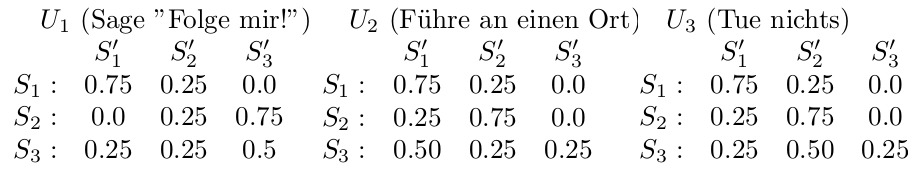
\includegraphics[width=0.6\linewidth]{figures/ch07_transmod-bsp.png}
		\caption{MDP Beispiel -- Transitionsmodell, Zeile muss Summe 1 haben, Spalten nicht (da Bias zu manchen Zuständen)}
		\label{fig:ch07:transmod-bsp}
	\end{figure}
\end{itemize}

\paragraph{Belohnungsmodell}
\begin{itemize}
	\item $R(s,u) = \text{Belohnung oder Strafe}$: wenn der Zustand $s$ war und der Agent f\"uhrt die Handlung $u$ aus, erh\"alt er die sofortige Belohnung (oder negativer Belohnung, also Strafe) wie vom Modell an $R(s,u)$ gegeben
	\item Das Belohnungsmodell ist eine Matrix
	\item Die Eintr\"age k\"onnen beliebige Realzahlen sein, je nach Modellierung
	\item Durch das Belohnungsmodell k\"onnen auch konkurrierende oder erg\"anzende Zielsetzungen modelliert werden
	\item Beispiel Museumsroboter: \textit{Sprechen} und \textit{Führen} kostet immer -1 Strafe, verglichen mit \textit{Tue nichts}, denn der Roboter ist faul und möchte Energie sparen, außerdem soll unnötige Unruhe im Museum vermieden werden. Einen folgenden Menschen an einen Ort zu führen gibt +5 Belohnung.
	\begin{figure}[!h]
		\centering
  		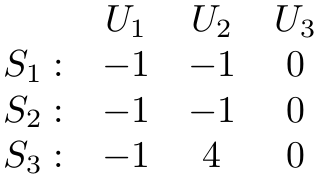
\includegraphics[width=0.2\linewidth]{figures/ch07_belmodel-bsp.png}
		\caption{MDP Beispiel -- Belohnungsmodell}
		\label{fig:ch07:belmodel-bsp}
	\end{figure}
\end{itemize}

\paragraph{Ziel des Agenten}
\begin{itemize}
	\item Das Ziel des rationalen Agenten im MDP ist, die Summe der Belohnungen bis zu einem bestimmten Zeithorizont (im reinen MDP meistens unendlich) zu maximieren
	\item Dies f\"uhrt zu einer \textbf{Gewinnmaximierung} bzw. \textbf{Risikoabsch\"atzung} in die Zukunft als Grundlage f\"ur den Entscheidungsprozess (zwischendurch negative Belohnung einzusammeln kann Sinn machen, Kosten in Kauf nehmen um langfristig große Belohnung einzusammeln; im Entscheidungsprozess müssen viele potentielle Handlungsketten gleichzeitig berücksichtigt werden)
	\item Das einzige explizite Ziel des Agenten ist die Gewinnmaximierung
	\item Sie bezieht implizit alle gegebenen Zielsetzungen in den Entscheidungsprozess mit ein
\end{itemize}

\paragraph{Gewinnmaximierung}
\begin{itemize}
	\item Da in einer stochastischen Welt keine festen Handlungsketten (in die Zukunft) existieren, wird eine Entscheidungsfunktion (\emph{policy}) berechnet
	\item Die Entscheidungsfunktion $\pi$ gibt f\"ur jeden Zustand $s$ eine Handlung zur\"uck: $\pi(s)$ (im klassischen MDP ist Entscheidungsfunktion eine Look-Up-Table)
	\begin{itemize}
		\ita deswegen wird in diesem Kontext meistens von \glqq entscheiden\grqq{} nicht wie z.B. in STRIPS von \glqq planen\grqq{} geredet (Planung ändert sich zu jedem Schritt)
	\end{itemize}
	\item Ein Agent in einem MDP muss nur eine optimale Entscheidungsfunktion $\pi^*$ berechnen, welche immer die Handlung mit der gr\"o{\ss}ten, langfristigen Gewinnerwartung w\"ahlt: $\pi^* (s)$
	\item Es gibt immer \textit{mindestens} eine $\pi^* (s)$, welche zu einem gegebenen MDP Modell optimale Entscheidungen liefert (selbst wenn es nur schlechte Möglichkeiten gibt und in der Praxis keinen Sinn mach)!
	\item Bei unendlichem Horizont ist die optimale Entscheidungsfunktion station\"ar: es gibt f\"ur einen Zustand immer dieselbe optimale Handlung. In einem voll beobachtbaren (reinen) MDP ist die Variante mit unendlichem Horizont somit die einfachste. Im Folgenden wird bei reinen MDPs nur der Fall des unendlichen Zeithorizonts ber\"ucksichtigt
\end{itemize}

\paragraph{Utility}
\begin{itemize}
	\item Die Utility einer Zustandskette ist die Summe ihrer Belohnungen bzw. Strafen:\\ $U_h(\left[s_0, s_1, s_2, \ldots \right]) = R(s_0) + R(s_1) + R(s_2) + \ldots$
	\item Die Einf\"uhrung eines Abschlagsfaktors (\emph{discount})  $\gamma \in \left[0,1\right]$ auf Zust\"ande  in der Zukunft erm\"oglicht eine endliche utility f\"ur alle unendlichen Zustandsketten (wie beim Menschen, Belohnung morgen ist mehr wert als Belohnung in einem Jahr):\\ $U_h(\left[s_0, s_1, s_2, \ldots \right]) = R(s_0) + \gamma R(s_1) + \gamma^2 R(s_2) + \ldots$\\
	Somit bildet sich eine Reihe welche asymptotisch konvergiert und das Problem der unendlichen Summe gelöst. $\gamma$ sollte aber nicht zu aggressiv gewählt werden
\end{itemize}

\paragraph{Entscheidungsfunktion}
\begin{itemize}
	\item Es existieren verschieden Verfahren, um eine optimale Entscheidungsfunktion aus dem gegebenen MDP Modell $(S, A, T, B)$ zu berechnen.
	Unter anderem: Policy Iteration oder Reinforcement Learning einer Policy (Gefahr hierbei: \glqq blinde Flecken\grqq{}der Policy)
	\item Das wichtigste aber ist: \textbf{Value Iteration} (zur Berechnung der optimalen Policy, bietet sich nur nicht an wenn Modellbildung im Vorfeld für Szenario zu schwierig ist)
\end{itemize}

\subsubsection{MDP Value Iteration}

\paragraph{Problem}
\begin{itemize}
	\item F\"ur jeden Zustand wird eine utility berechnet, die die \underline{erwartete utility} aller m\"oglichen, folgenden Zustandssequenzen widerspiegelt
	\item Daraus kann die Entscheidungsfunktion direkt gewonnen werden
	\item Die Zustandssequenzen wiederum h\"angen von der Entscheidungsfunktion ab
	\item $\Rightarrow$ verschr\"anktes Problem
\end{itemize}

\paragraph{Ansatz}
\begin{itemize}
	\item Iterativer Ansatz
	\item Die wirkliche utility eines Zustands w\"are die utility bezogen auf die optimale policy\\ $U_{real}(s) = U^{\pi^*}(s)$
	\item Die wirkliche utility ist jedoch zu Beginn nicht bekannt, da die optimale policy noch berechnet werden muss
	\item Zuerst wird eine beliebige policy $\pi_{start}$ gew\"ahlt
	\item Dazu wird jedem Zustand eine initiale utility zugewiesen
	\item Die tats\"achliche utility jedes Zustands, bezogen auf eine policy $\pi$, ist die Summe aller zuk\"unftigen Belohnungen:
	$U^{\pi}(s) = E \left[ \sum_{t = 0}^{\infty} \gamma^t R(s_t, u_t) | \pi, s_0 = s \right]$
	\item die Summe der zuk\"unftigen Belohnungen h\"angt jedoch von der Handlungswahl und damit von $\pi$ ab
\end{itemize}

\paragraph{Handlungswahl}
\begin{itemize}
	\item Es kann nun eine policy gefunden werden, die auf den aktuell zugewiesenen utilities basiert und I-Schritt weit optimal ist
	\item Nach der utility FUnktion wird nun die Handlung, die die erwartete zuk\"unftige Belohnung maximiert gew\"ahlt: $\pi^{1step*}(s) = argmax_u \sum_{s'} T(s', u, s) U(s')$
	\item Durch diese Formel wird auch ein Zusammenhang zwischen einem Zustand und seinem Nachbarn gebildet
\end{itemize}

\paragraph{Iterationsschritt}
\begin{itemize}
	\item Nun wird die Zuweisung wieder in die utility-Berechnung zur\"uckgef\"uhrt
	\item Es entsteht eine Iterationsformel zwischen benachbarten Zust\"anden:
	$U(s) = \gamma max_u (R(s,u) + \sum_{s'} T(s', u, s) U(s')) = \text{Bellmann Formel}$
	\item Somit kann r\"uckw\"arts von $\text{utility}(s)$ auf $\text{utility}(s')$ geschlossen werden
\end{itemize}

\paragraph{Iterationsablauf}
\begin{itemize}
	\item Beginn: irgendwelche niedrigen Werte f\"ur die utilites aller Zust\"ande
	\item Iterationsschritt: Anwendung der Bellmann Formel auf jeden Zustand unter Nutzung aller seiner Nachbarn
	\item Vielfache Anwendung des Iterationsschritts auf alle Zust\"ande
	\item Irgendwann wird ein Gleichgewicht erreicht, das die optimale policy $\pi^*$ ist
	\item Die Iteration konvergiert zur optimalen policy
	\item In der Praxis werden die Iterationen bis zu einer akzeptablen Konvergenzschranke durchgef\"uhrt
\end{itemize}

\paragraph{Algorithmus}
\begin{algorithm}
  \caption{MDP discreteValueIteration()
    \label{alg:vi}}
  \begin{algorithmic}[1]
    %\Require{$x$ and $y$ are packed \DNA strings of equal length $n$}
    %\Statex
    \Repeat 
      \For{ \textbf{each} state $s$ \textbf{in} $S$}
        \Let{$U^\prime(s)$}{$\gamma max_u(R(s,u)+\sum_{s^\prime}T(s^\prime,u,s)U(s^\prime))$}
      \EndFor
     \Until{convergence bound} \Comment{Änderung der utility-Werte zwischen zwei Schritten}
     \State \Return{$U$}
    %\EndFunction
  \end{algorithmic}
\end{algorithm}

Beispiel Museumsroboter:
\begin{itemize}
	\item Zustände: $S_1$=\textit{Kein Mensch}, $S_2$=\textit{Mensch, keine Intention zu folgen}, $S_3$=\textit{Mensch, Intention zu folgen} 
	\item Handlungen: $U_1$=\textit{Sage \glqq Folge mir!\grqq}, $U_2$=\textit{Führe an einen Ort}, $U_3$=\textit{Tue nichts}
	\begin{figure}[!h]
		\centering
  		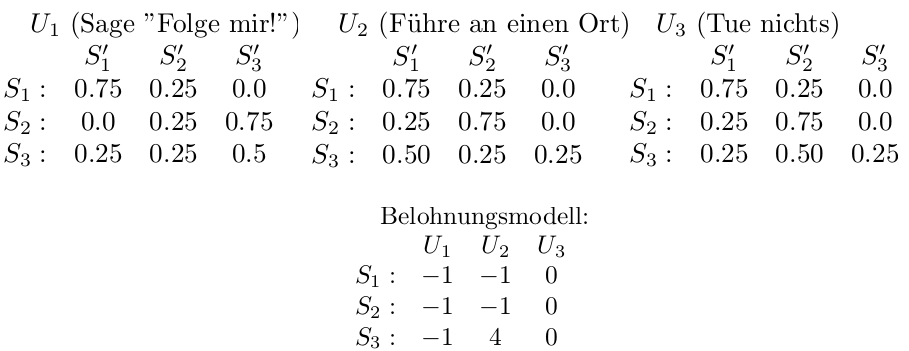
\includegraphics[width=0.6\linewidth]{figures/ch07_vi-bsp.png}
		\caption{MDP VI Beispiel -- Modell}
		\label{fig:ch07:vi-bsp}
	\end{figure}
	\item Initialisiere: $U(s_1=kein\text{ }Mensch) = -1$, $U(s_2=Mensch,\text{ }folgt\text{ }nicht) = -1$, $U(s_3=Mensch,\text{ }folgt) = -1$; wähle $\gamma = 0.9$
	\item $U(s)=\gamma max_u(R(s,u)+\sum_{s^\prime}T(s^\prime,u,s)U(s^\prime))$
	\begin{figure}[!h]
		\centering
  		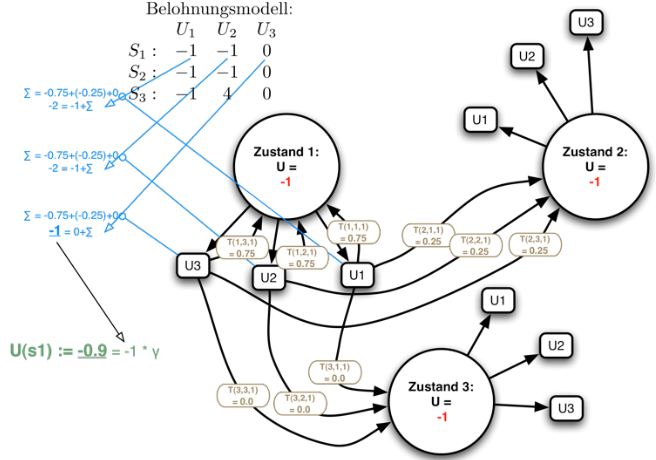
\includegraphics[width=0.45\linewidth]{figures/ch07_vi-bsp1.png}
		\caption{MDP VI Beispiel -- Iteration}
		\label{fig:ch07:vi-bsp1}
	\end{figure}
	\begin{figure}[!h]
		\centering
  		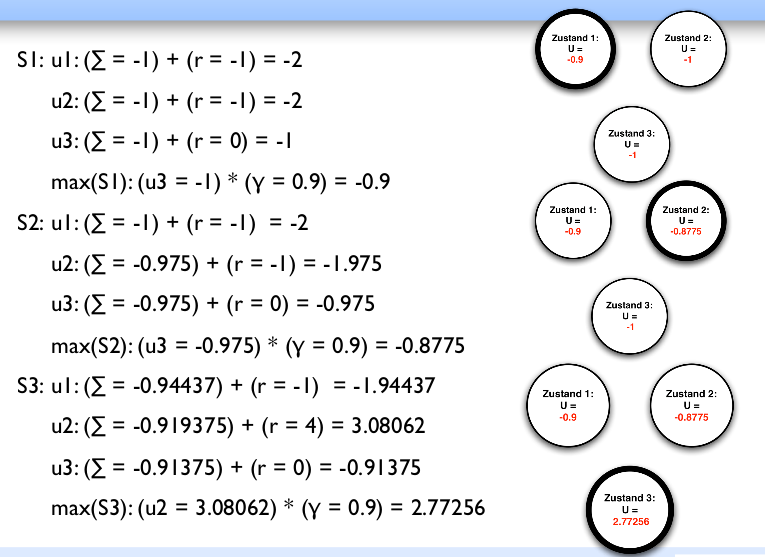
\includegraphics[width=0.65\linewidth]{figures/ch07_vi-bsp2.png}
		\caption{MDP VI Beispiel -- Iterationsschritt}
		\label{fig:ch07:vi-bsp2}
	\end{figure}
	\begin{figure}[!h]
		\centering
  		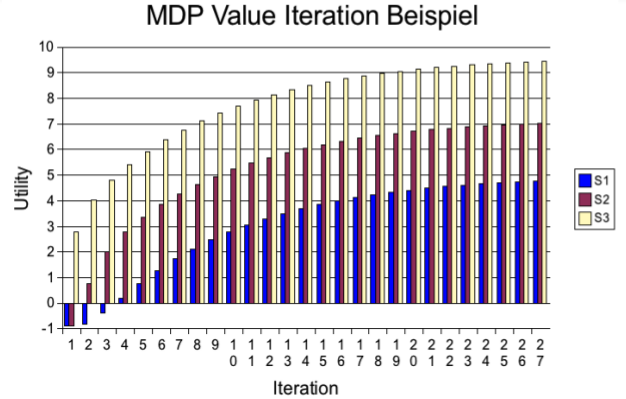
\includegraphics[width=0.45\linewidth]{figures/ch07_vi-bsp3.png}
  		\centering
		\caption{MDP VI Beispiel -- Ergebnis, \\$S_1: u_3$ am besten ab Iterationsschritt 1,\\ $S_2: u_1$ am besten ab Iterationsschritt 2\\ $S_3: u_2$ am besten ab Iterationsschritt 1}
		\label{fig:ch07:vi-bsp2}
	\end{figure}
\end{itemize}
\paragraph{Eigenschaften}
\begin{itemize}
	\item MDP Value Iteration ist eine Kontraktion: der Algorithmus konvergiert immer (auch wenn Modell keinen Sinn macht, dies muss vorher sicher gestellt werden)
	\item In der Praxis konvergiert er bei kleinerem $\gamma$ schneller
	\item MDP Value Iteration ist verh\"altnism\"a{\ss}ig schnell (im Vergleich zu anderen Verfahren und anderen Arten von MDPs)
	\item Fast optimale Entscheidungsfunktionen sind in der Praxis ausreichend
\end{itemize}

\subsubsection{MDP -- Schlussfolgerung}
\begin{itemize}
	\item Es gibt ein algorithmisches Konzept für optimale Entscheidungsfindung in stochastischen Umgebungen
	\item Ein rationaler Agent kann in Bezug auf Belohnungsmaximierung entscheiden
	\item Die (fast) optimale Belohnungsmaximierung ist berechenbar
	\item Die Modellierung eines Szenarios ist allerdings schwierig 
	\item Nur: Welche Umgebungseigenschaften decken reine MDPs ab?
\end{itemize}

\paragraph{Umgebungseigenschaften}
Markov Decision Processes sind ein theoretisches Rahmenwerk zur Modellierung von Entscheidungsfindung in
\begin{itemize}
	\item Dynamischen
	\item Sequenziellen
	\item Diskreten (aber auch kontinuierlichen)
	\item Stochastischen
	\item \textbf{Vollst\"andig} beobachtbaren (in Praxis meistens nicht gegeben, z.B. bei Serviceroboter)
	\item (Multiagent-)
\end{itemize}
Domänen.\\
Es gibt Erweitungen von MDPs für kontinuierliche Umgebungen (Zustände, Handlungen). Es gibt eine Erweiterung von MDPs für unvollständig beobachtbare Umgebungen: \textbf{Partially Observable Markov
Decision Processes}.

\subsection{POMDP (Partially Observable Markov Decision Processes)}
Eine Erweiterung von MDPs f\"ur unvollst\"andig beobachtbare Umgebungen. Perzeption ist \"ublicherweise verrauscht und deckt nur einen Teil des Szenarios ab. Beispielsweise Spracherkennung ist eine zentrale Fähigkeit für Serviceroboter (natürliche Mensch-Roboter-Interaktion), Sprache ist aber sehr verrauscht.

\paragraph{Zustandssch\"atzung}
\begin{itemize}
	\item Die Sch\"atzung des aktuellen Zustands muss nicht nur auf der Perzeption basieren
	\item Grundprinzip: rationaler Agent in Dom\"ane mit Markov Eigenschaft:
	\begin{itemize}
		\item Aktueller Zustand kann \"uber unvollkommene Perzeption \underline{beobachtet} werden (measurement)
		\item Aktueller Zustand kann auf Basis des vorherigen Zustands und der ausgef\"uhrten Handlung \underline{vorhergesagt} werden (prediction)
	\end{itemize}
	\item Die \textbf{Beobachtung} wird durch ein auf die Eigenschaften des physischen oder logischen Sensors abgestimmtes Unsicherheitsmodell abgebildet
	\item Die Unsicherheit kann so explizit, numerisch angegebenw erden
	\item Diese Unsicherheit kann verschieden modelliert werde:
	\begin{itemize}
		\item kontinuierlich oder diskret
		\item parametrisch oder nicht-parametrisch
	\end{itemize}
	\item Die \textbf{Vorhersage} wird \"uber ein Transitionsmodell realisiert
	\item Das Transitionsmodell f\"uhrt zu einer Wahrscheinlichkeitsverteilung \"uber allen Zust\"anden wie im MDP
	\item Eine Vorhersage funktioniert nur iterativ, ausgehend von einem aktuellen Zustand (bzw. begrenzten Historie: Markov Eigenschaft)
\end{itemize}

\paragraph{Bayes Filter} {\ }\\
Vorhersage und Beobachtung k\"onnen nun fusioniert werden, um zusammen eine h\"ohere Genauigkeit zu erreichen!\\

\textbf{Idee}:
\begin{itemize}
	\item Eine gute Vorhersage kann eine sehr ungenaue Beobachtung verbessern
	\item Eine gute Beobachtung pr\"azisiert jedoch eine ungenaue Vorhersage
	\item Da die Vorhersage nur iterativ funktioniert, arbeitet der Bayes Filter ebenfalls iterativ von Zeit $t-1$ nach $t$ 
\end{itemize}

\textbf{Zustandsvermutung}:
\begin{itemize}
	\item Die Ausgabe einer Vorhersage und auch einer Beobachtung ist eine Wahrscheinlichkeitsverteilung
	\item Da der Bayes Filter iterativ l\"auft, ist die Eingabe also auch eine Wahrscheinlichkeitsverteilung
	\item Der Agent besitzt daher zu jedem Zeitpunkt eine \underline{Zustandsvermutung} (belief)
	\item Die Zustandsvermutung repr\"asentiert die subjektive Wahrnehmung des Agenten bez\"uglich der nur unvollst\"andig beobachtbaren Welt (Zustandsraum)
	\item Die Zustandsvermutung ist eine
	\begin{itemize}
		\item diskrete Wahrscheinlichkeitsverteilung \"uber einem diskreten Zustandsraum
		\item oder eine kontinuierliche Verteilung \"uber einem kontinuierlichen Zustandsraum
	\end{itemize}
\end{itemize}
\begin{figure}[!h]
	\centering
  	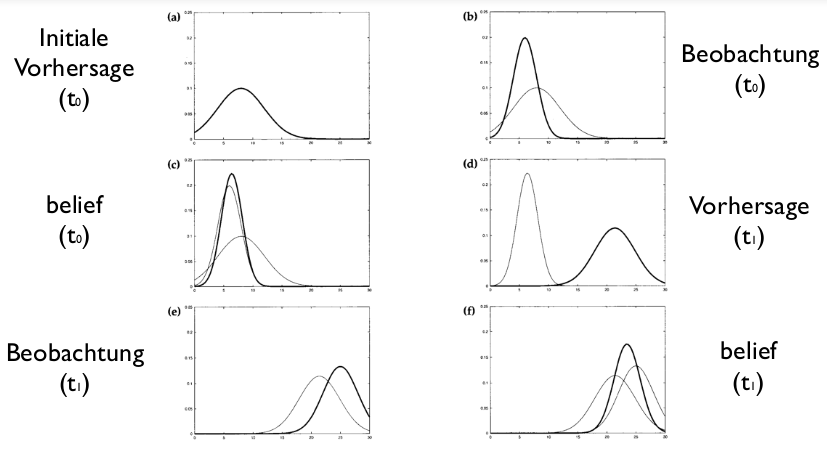
\includegraphics[width=0.8\linewidth]{figures/ch08_kont-bayes.png}
  	\centering
	\caption{Beispiel -- kontinuierlicher Bayesfilter}
	\label{kont-bayes}
\end{figure}
\textbf{Vorhersage}:
\begin{itemize}
	\item Zust\"ande $x$, Aktionen $u$
	\item Diskreter Fall: $\overline{p}_{k,t} = \sum_i p(X_t = x_k | u_t, X_{t-1} = x_i)p_{i, t-1}$
	\item Kontinuierlicher Fall: $\overline{bel}(x_t) = \int p(x_t | u_t, x_{t-1}) bel(x_{t-1})dx_{t-1}$
\end{itemize}

\textbf{Beobachtung}:
\begin{itemize}
	\item Zust\"ande $x$, Beobachtung $z$
	\item Diskreter Fall: $p_{k,t} = \eta p(z_t | X_t = x_k) \overline{p}(k,t)$
	\item Kontinuierlicher Fall: $bel(x_t) = \eta p(z_t | x_t) \overline{bel}(x_t)$
\end{itemize}

\textbf{Diskreter Bayes Filter}:\\
\autoref{fig:ch08:diskBayes}

\begin{figure}[h!]
\centering
\begin{subfigure}{.5\textwidth}
  \centering
  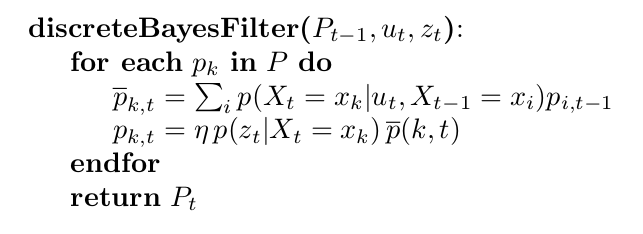
\includegraphics[width=\linewidth]{figures/ch08_diskreterBayes.png}
  \caption{Vollst\"andiger diskreter Bayes Filter mit Zust\"anden $x$, Aktion $u$ und Beobachtung $z$}
  \label{fig:sub1}
\end{subfigure}%
\begin{subfigure}{.5\textwidth}
  \centering
  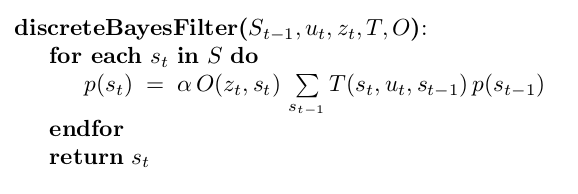
\includegraphics[width=\linewidth]{figures/ch08_diskreterBayesAlter.png}
  \caption{Alternative Darstellung mit Normalisierer $\alpha$, Zust\"anden $s$, explizitem Transitionsmodell $T$ und Beobachtungsmodell $O$}
  \label{fig:sub2}
\end{subfigure}
\caption{Diskreter Bayes Filter}
\label{fig:ch08:diskBayes}
\end{figure}

\textbf{Kontinuierlicher Bayes Filter}:\\
\autoref{fig:ch08:kontBayes}
\begin{figure}[h!]
	\centering
  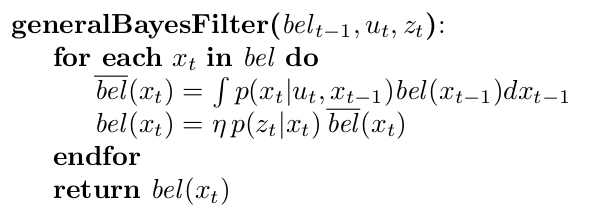
\includegraphics[width=0.5\linewidth]{figures/ch08_kontinuierlicherBayes.png}
\caption{Allgemeine kontinuierlicher Bayes Filter}
\label{fig:ch08:kontBayes}
\end{figure}
Kontinuierliche Bayes Filter werden durch spezielle Methoden realisiert.\\
Parametrische Filter:
\begin{itemize}
	\item Kalman Filter
	\item Extended Kalman Filter
	\item Unscented Kalman Filter
	\item Information Filter
	\item Extended Information Filter
\end{itemize}
Nicht-parametrische Filter: Partikelfilter\\ \\
\textbf{MDP + Bayes Filter}:\\
Um MDPs in einer unvollst\"andig beobachteten Umgebung nutzen zu k\"onnen werden Bayes Filter mit MDPs verbunden.
Das erfordert die Einf\"uhrung der Zustandsvermutung in den MDP.
Dadurch hat der MDP zwei Komponenten:
\begin{itemize}
	\item Realer Zustand der Welt
	\item Subjektive Zustandsvermutung des Agenten
\end{itemize}
$\Rightarrow$ \textbf{POMDPs}
\subsubsection{Eigenschaften und Ablauf von POMDPs}
POMDPs ermöglichen die Entscheidungsfindung in Domänen mit den Eigenschaften:
\begin{itemize}
	\item Dynamisch
	\item Sequentiell
	\item \underline{Diskret} oder Kontinuierlich
	\item Stochastisch
	\item \underline{Unvollst\"andig beobachtbar}
\end{itemize}

\paragraph{Struktur/Modell}
\begin{itemize}
	\item Eine Menge von symbolischen \textbf{Zust\"anden} der Welt $S$
	\item Eine Menge von symbolischen \textbf{Handlungen} des Agenten $U$
	\item Eine Menge von symbolischen \textbf{Beobachtungen} des Agenten $M$
	\item Ein \textbf{\"Ubergangsmodell} (transition model) $T(s', u, s)$ welches die stochastischen \"Uberg\"ange modelliert
	\item Ein \textbf{Belohnungsmodell} (reward model) $R(s,u)$ welches die Ziele und Absichten des Agenten modelliert
	\item Ein \textbf{Beobachtungsmodell} (observation model) $O(m, s')$ welches die Ungenauigkeit der Wahrnehmung des Agenten modelliert
	\item Einen Startzustand $s_0$
\end{itemize}

\paragraph{Statische Eigenschaften}
\begin{itemize}
	\item Die statischen Eigenschaften des reinen MDP gelten auch im POMDP
	\item Zusätzlich gilt: Der Agent kann in jedem Agentenzyklus \underline{genau eine} Beobachtung machen
	\item Weiterhin: In einem diskreten POMDP ist dies eine symbolische Beobachtung
	\item Im Folgenden wird von diskreten POMDPs ausgegangen
\end{itemize}

\paragraph{Dynamikmodelle}
\begin{itemize}
	\item Transitions- und Belohnungsmodell funktionieren wie beim MDP
	\item Hinzu kommt das Beobachtungsmodell:
	\begin{itemize}
		\item $O(m,s') =$ Wahrscheinlichkeit: wenn die Beobachtung $m$ gemacht wurde, dann ist die Wahrscheinlichkeit, dass der wirkliche Weltzustand $s'$ ist, vom Modell an $O(m,s'$ gegeben
		\item Das Beobachtungsmodell ist eine Matrix
	\end{itemize}
\end{itemize}

\paragraph{Sekund\"are Eigenschaften}
\begin{itemize}
	\item Die Entscheidungsfunktion (policy) existiert auch beim POMDP, wenn auch in anderer Form
	\item Hinzu kommt die Zustandsvermutung:
	\begin{itemize}
		\item Im diskreten Fall eine diskrete Wahrscheinlichkeitsverteilung \"uber alle Zust\"ande
		\item Die Zustandsvermutung wird zu jedem Zeitschritt durch Bayes Filterung neu berechnet
		\item F\"uhrt zu einer klaren Trennung zwischen objektiver Realit\"at (echter Weltzustand) und der subjektiven Sicht des Agenten
	\end{itemize}
\end{itemize}

\begin{figure}[!ht]
	\centering 
	\begin{subfigure}{.45\textwidth}
		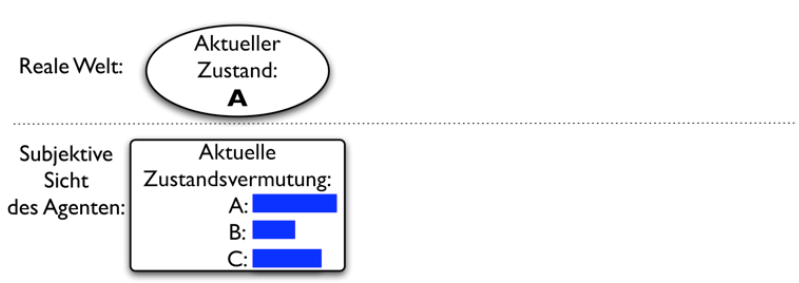
\includegraphics[width=\textwidth]{figures/ch08_pom.png}
		\caption{Beginn}
	\end{subfigure}
	\begin{subfigure}{.45\textwidth}
		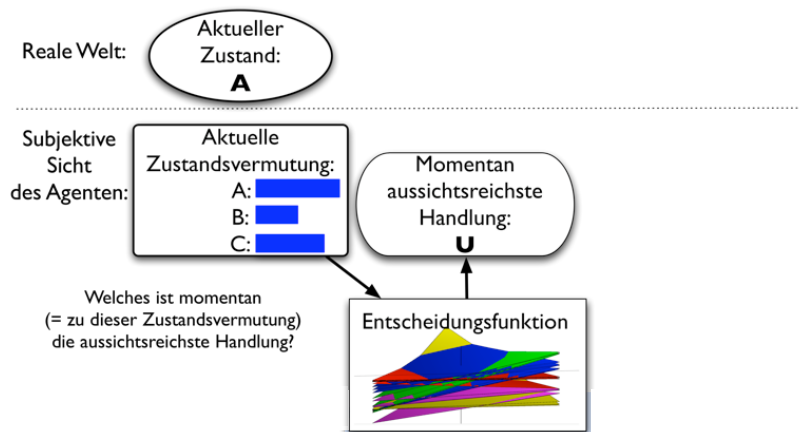
\includegraphics[width=\textwidth]{figures/ch08_pom1.png}
		\caption{Entscheidung}
	\end{subfigure}\\
	\begin{subfigure}{.45\textwidth}
		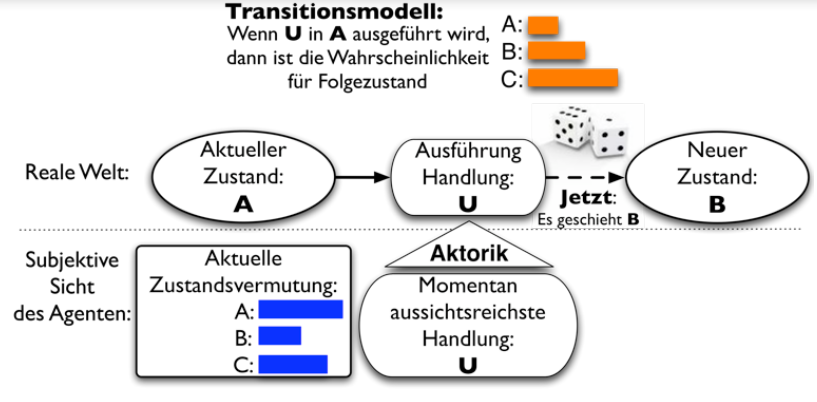
\includegraphics[width=\textwidth]{figures/ch08_pom2.png}
		\caption{Handlung}
	\end{subfigure}
	\begin{subfigure}{.45\textwidth}
		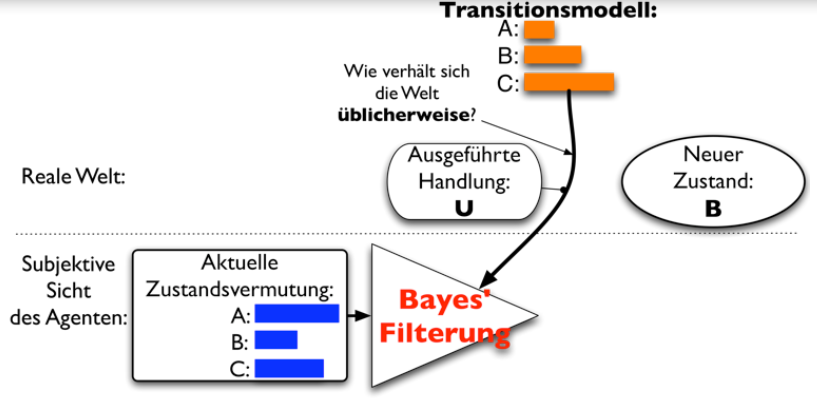
\includegraphics[width=\textwidth]{figures/ch08_pom3.png}
		\caption{Vorhersage}
	\end{subfigure}
	\begin{subfigure}{.45\textwidth}
		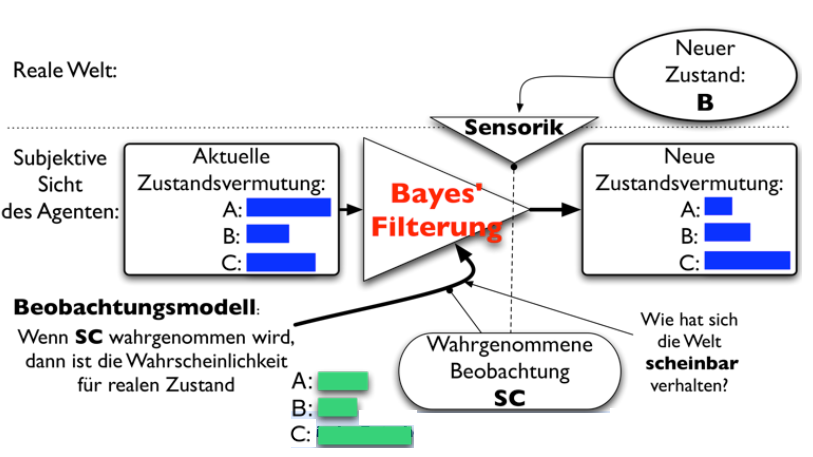
\includegraphics[width=\textwidth]{figures/ch08_pom4.png}
		\caption{Beobachtung}
	\end{subfigure}
	\caption{POMDP -- Schritte}
	\label{pom}
\end{figure}

\paragraph{Entscheidungsfunktion}
\begin{itemize}
	\item Bei MDPs enth\"alt die Entscheidungsfunktion eine Handlung zu jedem Zustand
	\item Im Gegensatz zu MDPs muss die Entscheidungsfunktion bei POMDPs \"uber \textbf{alle m\"oglichen Zustandsvermutungen} definiert sein
	\item Struktur der Entscheidungsfunktion
	\begin{itemize}
		\item Bei diskreten POMDPs: \"uber dem $|S|-1$ dimensionalen Raum \underline{aller m\"oglichen}\\ \underline{Zustandsvermutungen} definiert
		\item Bei kontinuierlichen POMDPs: \"uber einem unendlich-dimensionalen Raum definiert, daher speziell \"uber endlich-dimensionalen Teilr\"aumen angegeben
	\end{itemize}
	\item Berechnung der Entscheidungsfunktion: aufgrund der komplexen Struktur ist die Berechnung deutlich komplizierter als bei MDPs (Value Iteration existiert, ist aber anders)
\end{itemize}

\paragraph{Raum der Vermutungen (diskrete POMDP)}
\begin{itemize}
	\item Alle m\"oglichen Wahrscheinlichkeiten \"uber allen Zust\"anden $s$ eines Szenarios spannen den Raum der Zustandsvermutungen auf
	\item Da $\sum p(s_i) = 1$, ist der Raum begrenzt, also ein Simplex (= konvexe H\"ulle von $n+1$ Punkten in einem n-dimensionalen Raum)
	\item Wegen der Summe $|S|-1$ Dimensionen
	\item Beispiele in \autoref{raum}
	\begin{figure}[!h]
		\centering
  		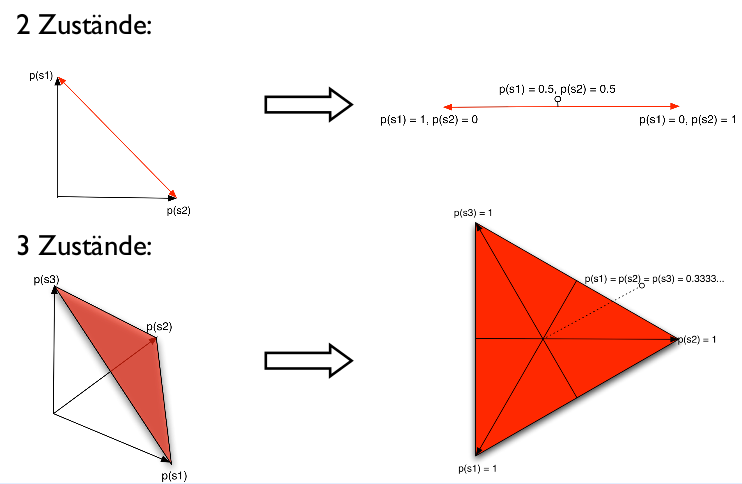
\includegraphics[width=0.5\linewidth]{figures/ch08_raum.png}
  		\centering
		\caption{Beispiel -- Raum der Vermutungen}
		\label{raum}
	\end{figure}
\end{itemize}
\newpage
\subsubsection{POMDP Value Iteration}
Aufgrund der komplexeren Struktur ist die Berechnung der Entscheidungsfunktion deutlich komplizierter als bei MDPs. Value Iteration existiert auch für POMDPs, funktioniert jedoch anders:
\begin{itemize}
	\item Iterativer Ansatz (wie bei MDP)
	\item Ein \underline{endlicher Horizont} wird vorausgesetzt
	\item Ein schrittweises Vorausschauen wird von einer initialen Entscheidungsfunktion aus durchgef\"uhrt
	\item Das Vorausschauen muss die stochastische Natur der Weltdynamik, als auch die verschieden genauen Beobachtungen eben dieser Dynamik in die Abw\"agung einflie{\ss}en lassen
\end{itemize}

\paragraph{Struktur}
\begin{itemize}
	\item Lineare Funktionen $\alpha$ repr\"asentieren die utility kontinuierlich \"uber dem gesamten Zustandsvermutungs-Simplex bezogen auf eine \underline{Handlung} (nicht Zustand, wie im MDP)
	\item F\"ur jede Zustandsvermutung kann aus den Funktionen eine utility berechnet werden
	\item Beispiele (\autoref{ch08:vi-bsp}):
	\begin{figure}[!h]
		\centering
  		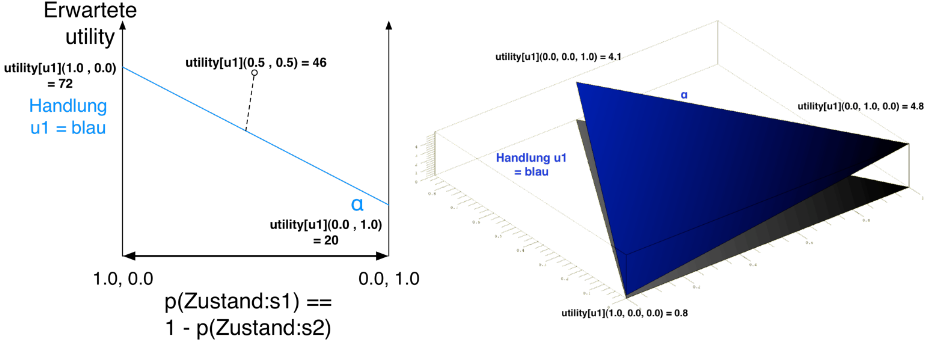
\includegraphics[width=0.6\linewidth]{figures/ch08_vi-bsp.png}
  		\centering
		\caption{POMDP VI Struktur -- Beispiele für 2 und 3 Zustände}
		\label{ch08:vi-bsp}
	\end{figure}
\end{itemize}

\paragraph{Beginn}
\begin{itemize}
	\item Der Algorithmus beginnt mit dem Pseudohorizont $0$
	\item Nun wird bis zu einem Horizont $T$ in die Zukunft iteriert
	\item Dabei wird eine Menge $\Gamma$ von linearen Funktionen $\alpha$ erzeugt, die Gewinnerwartungswerte f\"ur Mengen m\"oglicher Handlungsketten darstellen
\end{itemize}

\paragraph{Schritt} besteht aus zwei wesentlichen Teilen
\begin{enumerate}
	\item Tempor\"are Koeffizienten werden durch die Bayes Vorw\"artsfilterung (Projektion) jeder vorigen linearen Funktion \"uber jede m\"ogliche Handlung und Wahrnehmung erzeugt
	\begin{itemize}
		\item Die Projektion jeder linearen Funktion $\alpha$ aus $\Gamma$ in $t-1$ durch jede Kombination von Aktion $u$ und Beobachtung $m$ f\"uhrt zu den tempor\"aren Koeffizienten $v\{ k \}$ (siehe Code in \autoref{ch08:vi1})
		\begin{figure}[!h]
			\centering
  			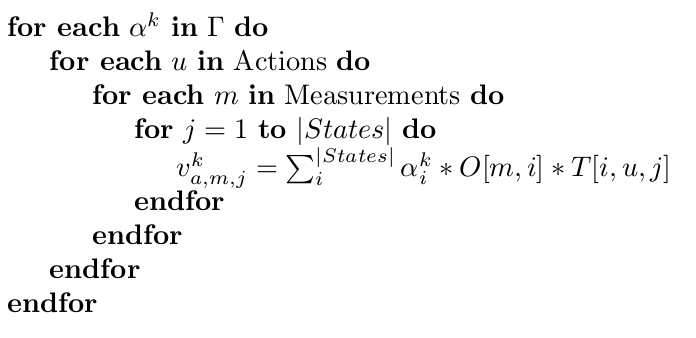
\includegraphics[width=0.4\linewidth]{figures/ch08_vi1.png}
  			\centering
			\caption{POMDP VI Schritt 1}
			\label{ch08:vi1}
		\end{figure}
	\end{itemize}
	\item Die tempor\"aren Koeffizienten werden f\"ur die Bildung der Erwartung \"uber alle m\"oglichen Beobachtungskombinationen verwendet, woraus die neuen linearen Funktionen erzeugt werden
	\begin{itemize}
		\item Aus den tempor\"aren Koeffizienten wird f\"ur jede m\"ogliche Kombination von Beobachtungen die Gewinnerwartung berechnet und eine neue lineare Funktion $\alpha'$ erzeugt (siehe Code in \autoref{ch08:vi2})
		\begin{figure}[!h]
			\centering
  			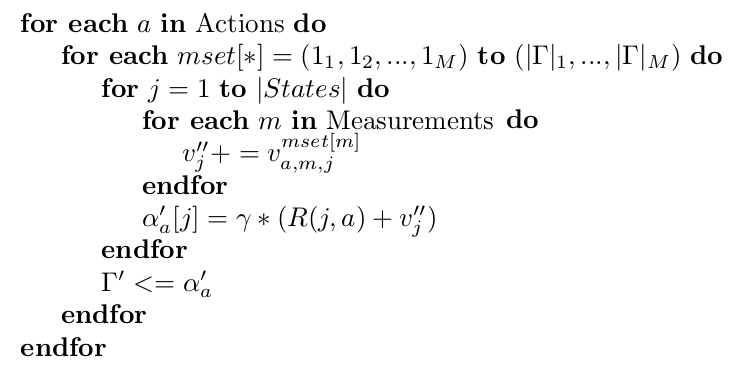
\includegraphics[width=0.4\linewidth]{figures/ch08_vi2.png}
  			\centering
			\caption{POMDP VI Schritt 2}
			\label{ch08:vi2}
		\end{figure}
	\end{itemize}
\end{enumerate}

\paragraph{Entscheidungsfunktion}
\begin{itemize}
	\item Die Entscheidungsfunktion ist das Maximum der utility in der Menge von linearen Funktionen \"uber dem jeweiligen Bereich des Zustandsvermutungsraums
	\item Diese Menge ist immer konvex \"uber dem Zustandsvermutungs-Simplex
	\begin{figure}[!h]
			\centering
  			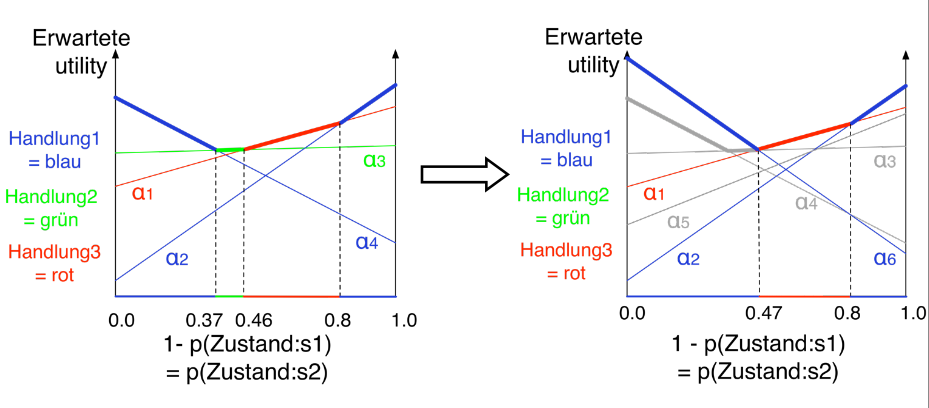
\includegraphics[width=0.7\linewidth]{figures/ch08_vi-bsp2.png}
  			\centering
			\caption{POMDP VI Schema; 2 Zustände, 3 Handlungen}
			\label{ch08:vi3}
	\end{figure}
\end{itemize}

\paragraph{Komplexit\"at}
\begin{itemize}
	\item Schritt Teil 2 ist aus komplexit\"atstheoretischer Sicht bedeutend:\\
	$\texttt{for each } mset\left[*\right] = (1_1, 1_2, \ldots, 1_M) \textbf{ to } (|\Gamma|_1, \ldots, |\Gamma|_M) \textbf{ do}$
	\item Hier geschieht eine kombinatorische Explosion bez\"uglich der Anzahl der erzeugten $\alpha$:\\
	$|\Gamma_t| = |Actions| * |\Gamma_{t-1}|^{|Observations|}$
	\item Was zu einer doppelt-exponentiellen Komplexit\"at (2-EXPSPACE) f\"uhrt:\\
	$|\Gamma| = |Actions|^{(\sum_{i=0}^{t-1} |Observations|^i)}$
	\newpage
	\item Beispiel 3 Aktionen, 3 Beobachtungen, $|\Gamma|$:
	\begin{itemize}
		\item Horizont $1:3$
		\item Horizont $2:81$
		\item Horizont $3:1594323$ 
		\item Horizont $4:1.2 \times 10^19$
		\item Horizont $5:5.4 \times 10^57$
	\end{itemize}
	\item[$\Rightarrow$] exakte POMDP Value Iteration unbrauchbar!!
	\item Um die Komplexit\"at handhabbar zu machen, wurden \textbf{approximative Value Iteration} Verfahren entwickelt. Dadurch wird meistens der Teil 2 des Iterationsschritts entsch\"arft. Alle relevanten Verfahren haben garantierte Fehlerschranken und zeichnen sich durch sehr gute Approximation aus
\end{itemize}

\paragraph{Point Based Value Iteration} als approximative Value Iteration
\begin{itemize}
	\item Nutzt ein dynamisches Raster zur Berechnung der Entscheidungsfunktion
	\item Die Entscheidungsfunktion wird nur f\"ur eine dynamische Menge von Stellvertreterpunkten im Zustandsvermutungsraum berechnet
	\item Sie gilt jedoch f\"ur den gesamten Raum
	\item Schema: Die Genauigkeit h\"angt in der Praxis von der Anzahl der Vertreterpunkte und der \"Anderungsh\"aufigkeit optimaler Handlungen \"uber dem Zustandsraum ab (vgl. \autoref{ch08:pbvi})
	\begin{figure}[!h]
			\centering
  			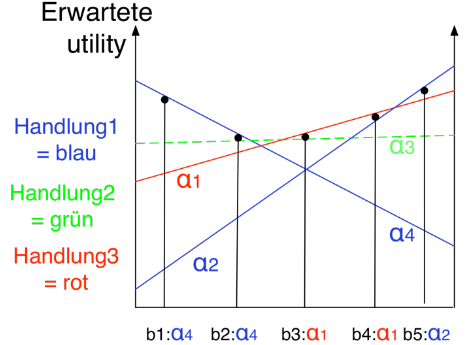
\includegraphics[width=0.4\linewidth]{figures/ch08_pbvi.png}
  			\centering
			\caption{PB VI Schema}
			\label{ch08:pbvi}
	\end{figure}
\end{itemize}
Weitere approximative Value Iterations sind PERSEUS, HSV12, SARSOP..

\subsubsection{POMDPs und Serviceroboter}
\begin{itemize}
	\item Die Nutzung von POMDPs in autonomen Servicerobotern steht noch ganz am Anfang
	\item Momentan fast nur in Simulationen und virtuellen Benchmarkszenarien im Einsatz
	\item Mono-Modale SLAM\footnote{Simultaneous Localization And Mapping (SLAM) ist eine zentrale Fähigkeit für autonome, mobile Roboter, also auch Serviceroboter}-Szenarien stehen dort noch im Mittelpunkt
	\item Die \"Ubertragung der Theorie auf Robotersteuerungen wird gerade erforscht. \autoref{ch08:einord} zeigt eine Einordnung aktueller Technologien.
		\begin{figure}[!h]
			\centering
  			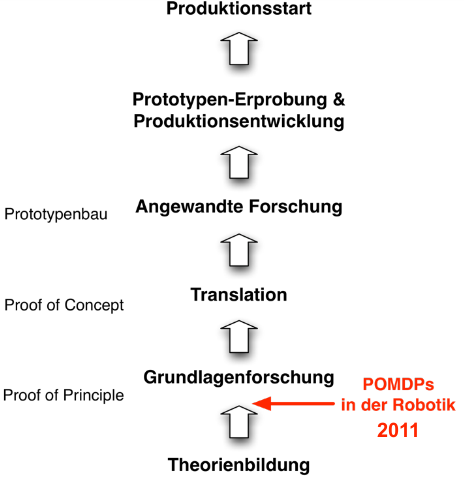
\includegraphics[width=0.3\linewidth]{figures/ch08_einord.png}
  			\centering
			\caption{POMDPs -- Technologieeinordnung}
			\label{ch08:einord}
	\end{figure}
	\item Herausforderungen
	\begin{itemize}
		\item \"Uberwindung der Abstraktionsl\"ucke zwischen Roboter Sensorik/Aktorik und symbolischen POMDPs
		\item stochastische Modellierung von Szenarien
		\item Strukturierung der stochastischen Modelle
		\item Integration der St\"arken klassischer Planung/Ausf\"uhrung
		\item Integration von maschinellem Lernen
	\end{itemize}
	\item POMDPs in einer Robotersteuerung (vgl. \autoref{fig:ch08_pomdpRobotersteuerung})
	\begin{figure}[h!]
		\centering
		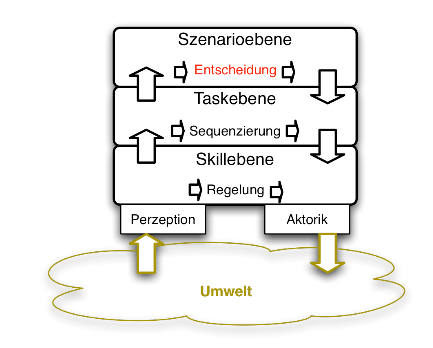
\includegraphics[width=0.4\textwidth]{figures/ch08_POMPDRobotersteuerung.png}
		\caption{POMDPs in einer Robotersteuerung}
		\label{fig:ch08_pomdpRobotersteuerung}
	\end{figure}
	\begin{itemize}
		\item POMDPs werden mit anderen Steuerungsmethoden zusammen eingesetzt
		\item Schichtung trennt die Methoden
	\end{itemize}
\end{itemize}